\subsection{Расчет потребления памяти iOS-клиентом}
\label{sec:eng:memory}

Для расчета потребления памяти iOS-клиентом будут использоваться стандартные инструменты Apple: \textit{Instruments} и~\textit{Xcode}. В~рамках данного ДП будет рассмотрено потребление памяти в~трёх состояних клиента и~оценён отпечаток в~памяти экрана настроек.

Первым рассматриваемым состоянием является экран выбора адреса сервера. К моменту показа этого экрана большая часть приложения всё ещё не загружена и~память потребляется в~основном сторонними библиотеками и~общими ресурсами. На~рисурке \ref{sec:eng:memory:initial} отображена статистика потребления памяти на~начальном экране, генерируемая \textit{Xcode}.

\begin{figure}[h]
  \centering
    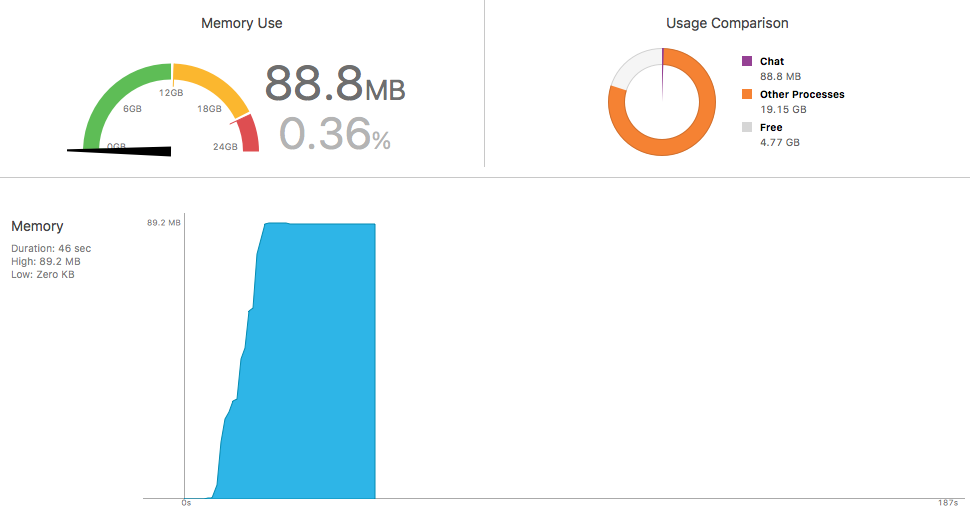
\includegraphics[width=1\textwidth]{inc/img/memory_initial.png}
  \caption{Потребление памяти iOS-клиентом на~начальном экране}
  \label{sec:eng:memory:initial}
\end{figure}

На рисунке \ref{sec:eng:memory:used} отражено количество потребляемой памяти после полной загрузки приложения и~показа экрана со списком всех диалогов. Как можно заметить, общий отпечаток в~памяти вырос примерно на~30 мегабайт, что существенно меньше начального скачка, обусловленного загрузкой сторонних библиотек.

\begin{figure}[h]
  \centering
    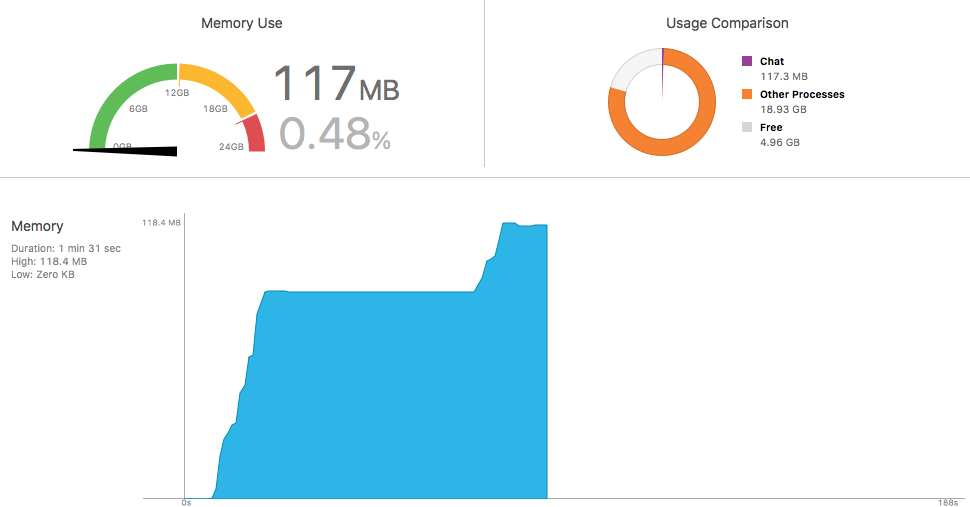
\includegraphics[width=1\textwidth]{inc/img/memory_used.png}
  \caption{Потребление памяти iOS-клиентом на~экране списка диалогов}
  \label{sec:eng:memory:used}
\end{figure}

\newcommand{\mcmd}{\text{П}_\text{д}}
\newcommand{\mcms}{\text{П}_\text{н}}
\newcommand{\mcmi}{\text{П}_\text{н}}
\newcommand{\mcmtd}{\text{П}_\text{2}}
\newcommand{\mcmts}{\text{П}_\text{3}}

Для расчета объёма памяти, выделевшейся при переходе на~экран списка диалогов, используется формула:
\begin{equation}\label{dialogueMemoryConsumptionEquation}
\mcmd = \mcmtd - \mcmi,
\end{equation}
\begin{explanation}
где & $ \mcmtd $ & количество потребляемой памяти, на~этапе открытия экрана диалогов, МБ; \\
    & $ \mcmi $ & количество потребляемой памяти, после запуска клиента, МБ.
\end{explanation}

Рассчитаем объём потребляемой экраном списка диалогов памяти, подставив значения в~формулу (\ref{dialogueMemoryConsumptionEquation}):
\begin{center}
\(\mcmd = \num{117} - \num{88.8} = \num{28.2} \, \text{МБ}\)
\end{center}

Для расчета объёма памяти, выделившейся при переходе на~экран настроек, используется формула:
\begin{equation}\label{settingsMemoryConsumptionEquation}
\mcms = \mcmts - \mcmtd,
\end{equation}
\begin{explanation}
где & $ \mcmts $ & количество потребляемой памяти, на~этапе открытия экрана диалогов, МБ; \\
    & $ \mcmtd $ & количество потребляемой памяти, на~этапе открытия экрана настроек, МБ.
\end{explanation}

Стоит отметить, что полученное значение отражает потребление памяти не только экраном, но сервисами приложения, инициализирующихся при переходе из~начального состояния приложения в~рабочее.

Рассчитаем объём памяти, потребляемой экраном настроек, подставив значения в~формулу (\ref{settingsMemoryConsumptionEquation}):
\begin{center}
\(\mcmd = \num{119} - \num{117} = \num{2} \, \text{МБ}\)
\end{center}

\textit{Xcode} хорошо подходит для~беглого аудита потребления ресурсов клиентом, однако имеет ряд недостатков:

\begin{itemize}
	\item завышает значения в~сравнении с~потреблением ресурсов на~настоящем устройстве;
	\item даёт малое количество информации;
	\item не даёт способов как-либо повлиять на~алгоритм сбора данных, отфильтровать шумы.
\end{itemize}

Для серьёзного профилирования вместе с~\textit{Xcode} поставляется приложение \textit{Instruments}, которое позволяет детально рассмотреть огромное количество метрик для~клиентов под~операционные системы Apple. В~рамках данного дипломного проектирования, интересующим инструментов является монитор аллокаций, который позволяет:

\begin{itemize}
	\item отслеживать общее потребление памяти во времени;
	\item отслеживать изменение потребления памяти между определёнными событиями или произвольными моментами времени;
	\item просмотреть весь граф объектов, находящийся в~данный момент в~памяти или на~стеке;
	\item проанализировать природу появления объекта и~причины, по~которым он не может освободить память;
	\item автоматически определять утечки памяти.
\end{itemize}

Для тестирования был выбран экран настроек приложения, на~рисунке \ref{sec:eng:memory:generations} приведены результаты замеров, где:

\begin{explanation}
где & \textit{Generation A} & начальное поколение приложения, которое появляется в~результате запуска; \\
    & \textit{Generation B} & поколение объектов, появившихся в~результате показа экрана настроек; \\
    & \textit{Generation C} & поколение объектов, появившихся в~результате закрытия экрана настроек; \\
    & \textit{Generation D} & поколение объектов, появившихся в~результате повторного показа экрана настроек. \\
\end{explanation}

\begin{figure}[h]
  \centering
    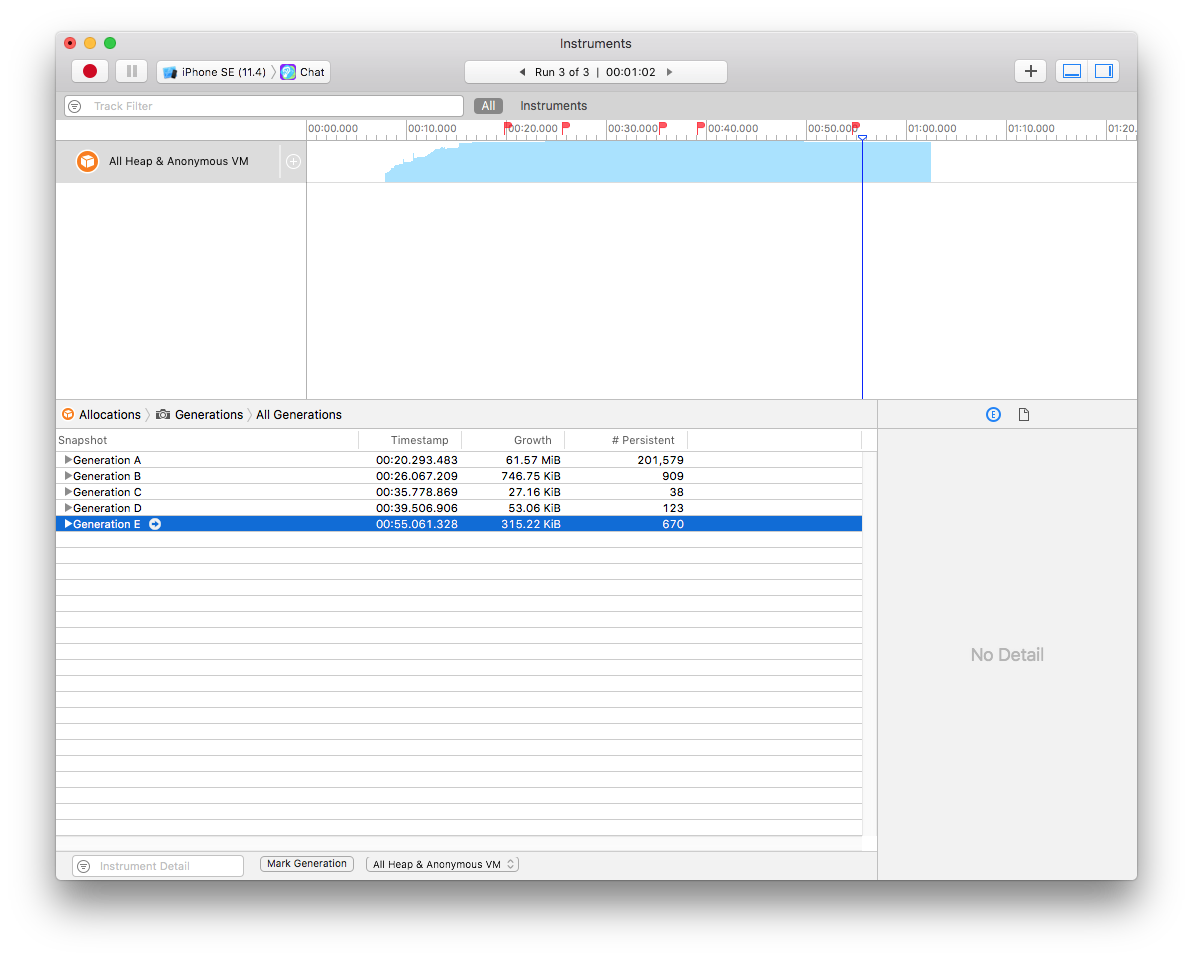
\includegraphics[width=1\textwidth]{inc/img/memory_generations.png}
  \caption{Потребление памяти iOS-клиентом в~процессе работы с~экраном настроек}
  \label{sec:eng:memory:generations}
\end{figure}

\begin{table}[h!]
\caption{Результат замеров потребления памяти iOS-клиентом}
\label{sec:eng:memory:result}
\centering
\begin{tabularx}{\textwidth}{ |X|X| } 
 \hline
 \emph{Начальный экран} & \num{88.8} Мегабайт \\ 
 \hline
 \emph{Экран диалогов} & \num{117} Мегабайт \\ 
 \hline
 \emph{Прирост на~экране диалогов} & \num{28.2} Мегабайт \\ 
 \hline
 \emph{Экран настроек} & \num{119} Мегабайт \\ 
 \hline
 \emph{Прирост на~экране настроек} & \num{2} Мегабайта \\ 
 \hline
\end{tabularx}
\end{table}

В таблице \ref{sec:eng:memory:result} отражены результаты расчетов в~текущем разделе. Как можно заметить, при закрытии экрана настроек не освобождается достаточное количество памяти, а~при повторном открытии -- выделяется очень мало памяти. Это свидетельствует об утечки памяти, однако в~данном случае частично утечка обусловлена наличием кэша на~экране, который являтеся общим на~приложении и~очищается только при получении запроса от~операционной системы. Основным потребителем памяти в~приложении являются сторонние библиотеки, поэтому на~этапе поддержки приложения будет произведён пересмотр используемх библиотек с~возможной заменой или оптимизацией.